\documentclass[12pt]{article}
\usepackage[english]{babel}
\usepackage{natbib}
\usepackage{url}
\usepackage[utf8x]{inputenc}
\usepackage{amsmath}
\usepackage{graphicx}
\graphicspath{{images/}}
\usepackage{parskip}
\usepackage{fancyhdr}
\usepackage{vmargin}
\usepackage{subfig}
\usepackage{float}
\setmarginsrb{3 cm}{2.5 cm}{3 cm}{2.5 cm}{1 cm}{1.5 cm}{1 cm}{1.5 cm}

\title{5 - Operational Amplifier (Prelab)}                             % Title
\author{John Wu \\ Ian Smith \\ Bilal Yousuf}                               % Author
\date{\today}                                                           % Date

\makeatletter
\let\thetitle\@title
\let\theauthor\@author
\let\thedate\@date
\makeatother

\pagestyle{fancy}
\fancyhf{}
\rhead{\theauthor}
\lhead{\thetitle}
\cfoot{\thepage}

\begin{document}

%%%%%%%%%%%%%%%%%%%%%%%%%%%%%%%%%%%%%%%%%%%%%%%%%%%%%%%%%%%%%%%%%%%%%%%%%%%%%%%%%%%%%%%%%

\begin{titlepage}
    \centering
    \vspace*{0.5 cm}
    
\includegraphics[scale = 0.07]{mcgill-logo.png}\\[1.0 cm]   % University Logo
    \textsc{\LARGE McGill University}\\[1.0 cm]   % University Name
    \textsc{\Large ECSE 335}\\[0.5 cm]               % Course Code
    \textsc{\large Microelectronic Labs}\\[0.5 cm]               % Course Name
    \rule{\linewidth}{0.2 mm} \\[0.4 cm]
    { \huge \bfseries \thetitle}\\
    \rule{\linewidth}{0.2 mm} \\[1.5 cm]
    \begin{minipage}{0.4\textwidth}
        \begin{flushleft} \large
            \emph{Authors (Group 14):}\\
            \theauthor
            \end{flushleft}
            \end{minipage}~
            \begin{minipage}{0.4\textwidth}
            \begin{flushright} \large
            \emph{Student Number:} \\
            260612056 \\ 260634831 \\ 260680182                                  % Your Student Number
        \end{flushright}
    \end{minipage}\\[2 cm]
 
    {\large \thedate}\\[2 cm]
 
    \vfill
    
\end{titlepage}

%%%%%%%%%%%%%%%%%%%%%%%%%%%%%%%%%%%%%%%%%%%%%%%%%%%%%%%%%%%%%%%%%%%%%%%%%%%%%%%%%%%%%%%%%

\section*{5.1 Preparation}

In this section, the active load differential amplifier, the buffer stage and the Class AB 
output stage will be combined as shown in Figure 1.1 in order to yield an operational 
amplifier with an open-loop gain of around 2500V/V. Also, the amplifier’s stability will 
be investigated, compensation will be performed if needed, and finally, the circuit will 
be used in a closed-loop feedback configuration.

\subsection*{5.1.2 Combine the active load differential amplifier, buffer stage, and 
Class AB output stage together and load them with a 330 $\Omega$ resistor. Ensure that the 
combination of the circuits yields the expected results from Spice simulations. Document 
the frequency response, gain, voltage transfer characteristic, and maximal input and 
output ranges. Make sure that the DC point at the output is 0V. Why is that critical in 
the context of feedback? Ensure that the parasitic capacitors are still accounted for. }

ANSWER HERE

\begin{figure}[H]
    \centering
    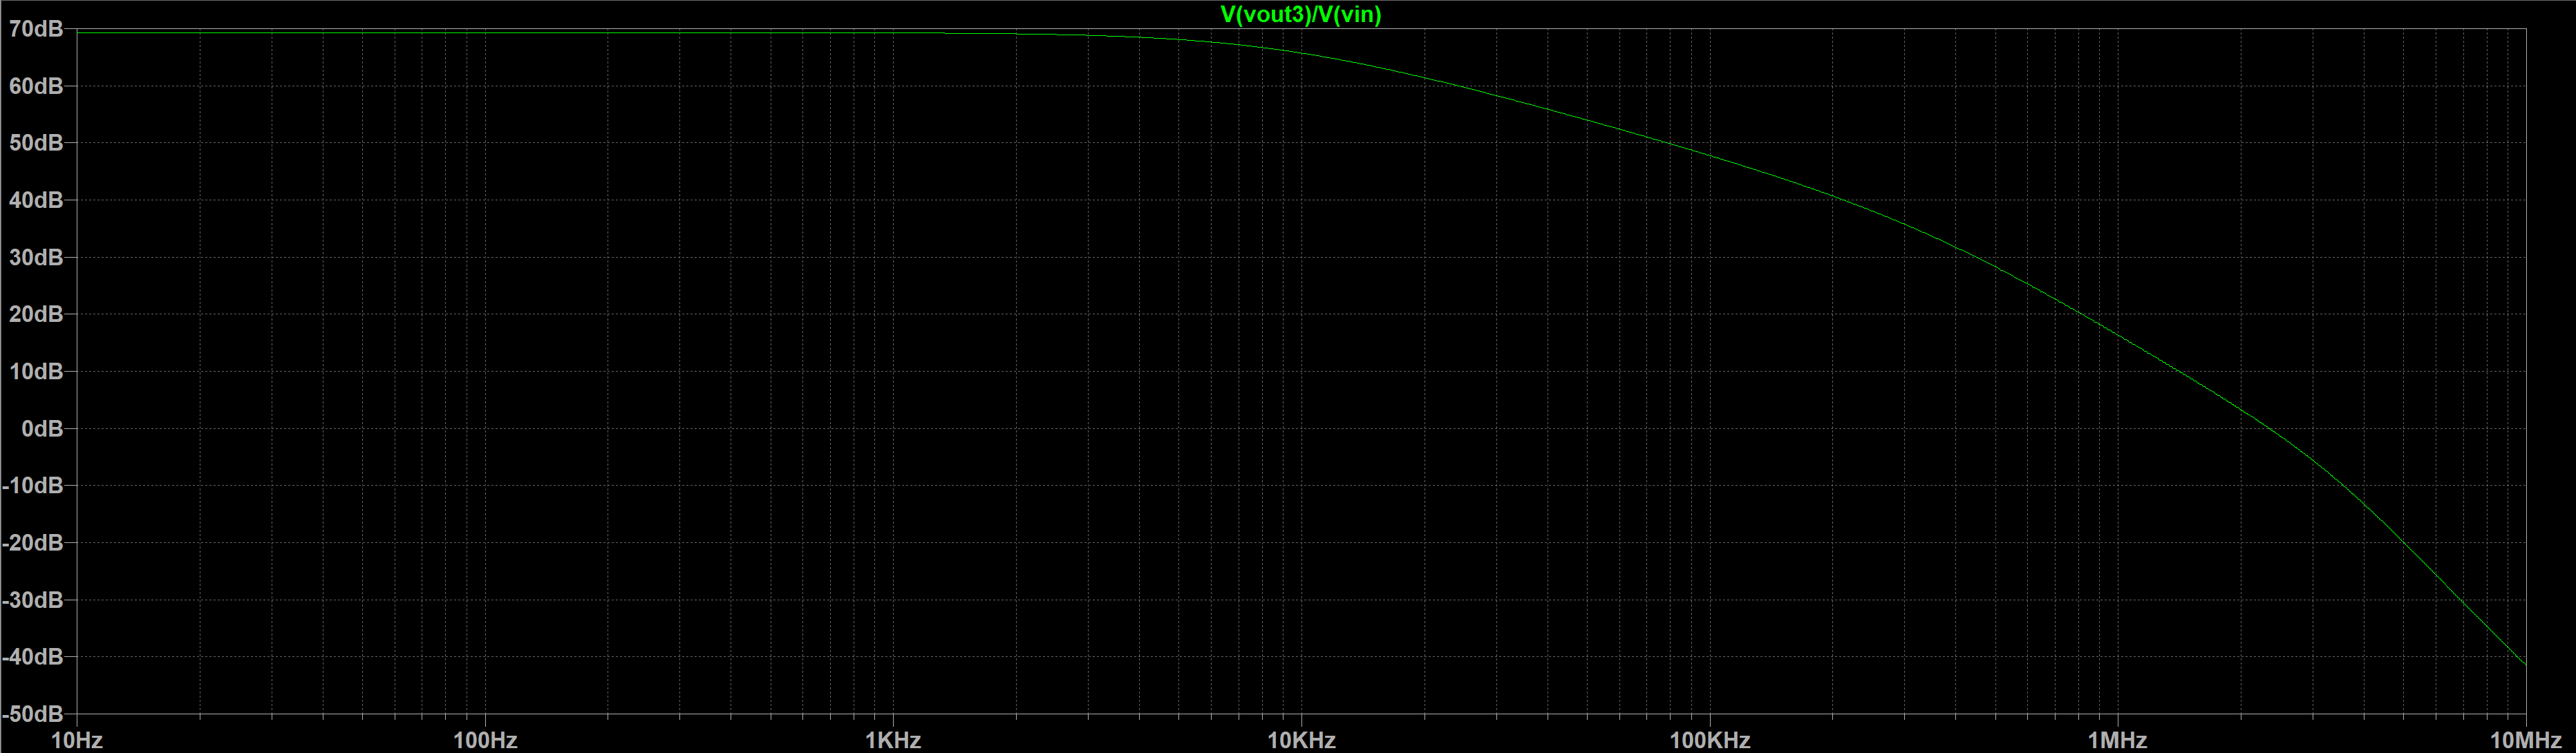
\includegraphics[width=1.0\textwidth]{512.1.PNG}
    \caption{Diagram example}
\end{figure}
    

\subsection*{5.1.3 Determine the phase margin of the circuit.}

The phase margin of the circuit is $180 -  |phase_{0dB}| = 180 - 90 = 90º$.

\subsection*{5.1.4 By examining the circuit diagram, determine where a 
compensating capacitor could be added to increase the phase margin of the circuit. 
You may use which ever compensating method you deem reasonable. Hint: Remember that, 
in its simplest form, compensating is equivalent to slowing down a circuit’s frequency 
response to increase its phase margin.}

Through examination of the circuit, a compensating capacitor can be added in parallel with the $330\Omega$ load to increase the phase margin of the circuit.

\subsection*{5.1.5 If needed, compensate the circuit to yield a minimum phase margin of 25 degrees.  }

The phase margin of the circuit is 90º which is larger than the required minimum of 25º therefore the circuit does not need to be compensated further.

\subsection*{5.1.6 Load the circuit with a 330 $\Omega$ resistor. Document the frequency response, 
voltage transfer characteristic, time response, and maximal input and output ranges. 
Hint: You may decouple the load with a capacitor if you have problems.}

ANSWER HERE

\subsection*{5.1.7 Design a non-inverting feedback amplifier which provides a gain of 150V/V. 
Do not assume the open-loop gain to be infinite in this case, but use your measured open loop 
gain value. Provide a schematic of the design. Plot the frequency response, time response, and 
voltage transfer characteristic of this design. }

Using the closed loop gain equations along with the equation for the feedback loop gain, we can determine the values of R1 and R2 needed in the feedback loop.
\newline
$A_closed  = \frac{A_open}{1 + A\beta}\\
\\
150 = \frac{3162}{1 + 3162\beta}\\
\\
\beta = 0.00635\\
\\
\beta = \frac{R_1}{R_1 + R_2}\\
\\
0.00635(R_1 + R_2) = R_1\\
\\
0.9936R_1 = 0.00635R_2\\
\\
R_2 = 1k\Omega, R_1 = 156k\Omega
$

\subsection*{5.1.8 Comment on the effect of the feedback loop on the characteristics of the 
amplifier. Mainly, comment on the bandwidth, gain, and input resistance.}

The negative feedback loop would affect various parameters of the amplifier:
\begin{enumerate}
\item
The bandwidth increases, while the gain decreases (the bandwidth-product remains constant)
\item
The input resistance of the circuit increases, since we are using a series-shunt configuration.
\item
The gain becomes less sensitive to input changes, stays constant at the desired value of 150V/V.
\end{enumerate}

\subsection*{5.1.9 What are the advantages and disadvantages of feedback in this case?}

Once again, a higher input resistance and a higher bandwidth seem to be the main advantages of the circuit, due to the stability provided by the negative feedback network. However, the main disadvantage is the lower in-band gain provided by the circui


\end{document}